\documentclass[aspectratio=169,10pt]{beamer}

\usepackage[T1]{fontenc}
\usepackage[utf8]{inputenc}
\usepackage[english]{babel}
\usepackage{booktabs}
\usepackage{graphicx}
\usepackage{tikz}
\usetikzlibrary{arrows.meta,positioning,fit,backgrounds,calc}
\usepackage{pgfplots}
\pgfplotsset{compat=1.18}

% --------------------------------------------------
% Theme: the IMEKO TC4 2026 deck (metropolis tuned to the CTU palette), reused.
%   * frame title in a solid CTU-blue bar, thin red progress bar under it
%   * Fira Sans (pdflatex build via the `fira` package) + newtxsf for sans math
%   * one accent colour (red), reserved for the waveform-trained model and the
%     highlighted result -- the rest of the data is in greys
% --------------------------------------------------
\usetheme[progressbar=frametitle,numbering=fraction,block=fill,sectionpage=none]{metropolis}
\usepackage[sfdefault,lining]{FiraSans}
\usepackage{FiraMono}
\usepackage{newtxsf}
\usepackage{fontawesome5}
% Stop the frame count (and the progress bar) at the last main frame.
\usepackage{appendixnumberbeamer}

% Notes build: slides-notes.tex sets \SHOWNOTES and \input's this file, so the
% spoken script lives in exactly one place -- the \note{} blocks below.
\usepackage{pgfpages}
\ifdefined\SHOWNOTES\setbeameroption{show only notes}\fi

\definecolor{ctublue}{RGB}{0,101,189}
\definecolor{ctunavy}{RGB}{0,55,110}
\definecolor{accent}{RGB}{200,16,46}
\definecolor{ink}{RGB}{35,38,45}
\definecolor{paper}{RGB}{255,255,255}
\definecolor{panel}{RGB}{240,244,249}
\definecolor{gray1}{HTML}{3D414B}
\definecolor{gray2}{HTML}{767B86}
\definecolor{gray3}{HTML}{AEB2BA}

\setbeamercolor{normal text}{fg=ink,bg=paper}
\setbeamercolor{structure}{fg=ctublue}
\setbeamercolor{alerted text}{fg=accent}
\setbeamercolor{example text}{fg=ctublue}
\setbeamercolor{frametitle}{fg=paper,bg=ctublue}
\setbeamercolor{progress bar}{fg=accent,bg=ctublue!30}
\setbeamercolor{progress bar in head/foot}{fg=accent,bg=ctublue!30}
\setbeamercolor{block title}{fg=ctublue,bg=panel}
\setbeamercolor{block body}{bg=panel}
\setbeamercolor{block title alerted}{fg=paper,bg=accent}
\setbeamercolor{block body alerted}{bg=accent!8}
\setbeamercolor{footline}{fg=ink!55}
\setbeamercolor{page number in head/foot}{fg=ink!55}
\setbeamercolor{title}{fg=paper}
\setbeamercolor{subtitle}{fg=paper}
\setbeamercolor{author}{fg=paper}
\setbeamercolor{institute}{fg=paper}
\setbeamercolor{date}{fg=paper}

\setbeamerfont{frametitle}{size=\large,series=\bfseries}
\setbeamerfont{block title}{series=\bfseries}
\setbeamerfont{footline}{size=\scriptsize}
\setbeamerfont{page number in head/foot}{size=\scriptsize}
\setbeamerfont{title}{size=\LARGE,series=\bfseries}
\setbeamerfont{author}{size=\normalsize}
\setbeamerfont{institute}{size=\small}
\setbeamerfont{date}{size=\small}

\setbeamertemplate{navigation symbols}{}
\setbeamertemplate{itemize items}{\textcolor{ctublue}{\raisebox{0.15ex}{\rule{0.7ex}{0.7ex}}}}
\setbeamertemplate{enumerate items}[default]
\setbeamertemplate{frame footer}{\insertshorttitle\ \textperiodcentered\ BEC 2026}
\setbeamercovered{transparent=25}
\metroset{progressbar=frametitle}
\makeatletter
\setlength{\metropolis@progressinheadfoot@linewidth}{1.2pt}
\setlength{\metropolis@frametitle@padding}{1.5ex}
\makeatother

% the one highlight colour: the deployed (waveform-trained) model, the headline numbers
\newcommand{\hl}[1]{\textbf{\color{accent}#1}}

% Icon tile for the motivation slide: \fnode{x}{icon}{label}{sub-caption}
\newcommand{\fnode}[4]{\node[text width=40mm,align=center,inner sep=0pt] at (#1,0)
  {{\color{ctublue}\Large #2}\\[2pt]{\small\bfseries #3}\\[1pt]{\scriptsize\color{ink!65}#4}};}

% Results charts: MCC (or P/R) over the SNR levels, categorical x axis.
\pgfplotsset{
  snrslide/.style={
    width=0.80\textwidth,height=0.43\textwidth,
    ymin=0.2,ymax=1.04,
    ytick={0.2,0.4,0.6,0.8,1.0},
    yticklabel style={/pgf/number format/fixed,/pgf/number format/precision=1},
    tick label style={font=\scriptsize,color=ink!70},
    label style={font=\scriptsize,color=ink!70},
    axis line style={draw=none},
    tick style={draw=none},
    ymajorgrids,grid style={ink!12,line width=0.4pt},
    clip=false,
    every axis plot/.append style={line width=1pt,mark=*,mark size=1.6pt},
  },
  dim/.style={color=#1,mark options={fill=#1}},
  hot/.style={color=accent,line width=1.8pt,mark size=2.2pt,mark options={fill=accent}},
}
\tikzset{lbl/.style={font=\scriptsize,anchor=west,xshift=3pt,color=#1}}


% "Two ways to train for noise": block diagram with a summing junction and a noise source.
\tikzset{
  twoways/.style={
    blk/.style={draw=ctublue,thick,rounded corners,fill=ctublue!8,
                minimum height=7.5mm,text width=17mm,font=\small,align=center},
    ar/.style={-{Latex[length=1.8mm]},draw=gray,semithick},
    why/.style={font=\scriptsize,text width=40mm,align=left,anchor=west,color=ink!80}},
  sum/.style={draw=#1,thick,circle,fill=paper,minimum size=5.5mm,inner sep=0pt,
              path picture={\draw[#1,thick]
                ($(path picture bounding box.center)+(-1.6mm,0)$) -- ++(3.2mm,0)
                ($(path picture bounding box.center)+(0,-1.6mm)$) -- ++(0,3.2mm);}},
  src/.style={draw=#1,thick,rounded corners,fill=paper,minimum width=16mm,minimum height=5.5mm},
  card/.style={draw=#1,thick,rounded corners,inner xsep=4mm,inner ysep=2.2mm},
  head/.style={fill=#1,text=paper,font=\small\bfseries,rounded corners,
               inner xsep=2.5mm,inner ysep=1.2mm,anchor=west},
}
% noise source glyph: \noisesrc{name}{coordinate}{colour} -- a random-looking trace in a box
\newcommand{\noisesrc}[3]{%
  \node[src=#3] (#1) at (#2) {};
  \begin{scope}[shift={(#1.center)},x=1mm,y=1mm]
    \draw[#3,line width=0.5pt,line join=round]
      (-6,0) -- (-5.4,1.6) -- (-4.8,-1.1) -- (-4.2,0.7) -- (-3.6,-1.8) -- (-3,1.2)
      -- (-2.4,-0.4) -- (-1.8,1.9) -- (-1.2,-1.4) -- (-0.6,0.5) -- (0,-0.9)
      -- (0.6,1.5) -- (1.2,-1.7) -- (1.8,0.3) -- (2.4,1.1) -- (3,-1.3) -- (3.6,0.8)
      -- (4.2,-0.5) -- (4.8,1.7) -- (5.4,-1.0) -- (6,0.2);
  \end{scope}}

% --------------------------------------------------

\title[Post-Trigger Artillery Launch Classifier]{A Lightweight Noise-Robust Post-Trigger\\Classifier for Embedded Acoustic\\Artillery Launch Detection}
\author{\underline{Martin Maxa} \and Jakub Svatoš \and Jakub Zelinka}
\institute{Czech Technical University in Prague\\Faculty of Electrical Engineering, Department of Measurement}
% TODO: exact day and session of the talk, once the programme is out.
\date{BEC 2026 -- Baltic Electronics Conference\\[5pt]
      Tallinn, Estonia \textperiodcentered\ October 2026}

\begin{document}


\begin{frame}[plain,noframenumbering]
  % Full-bleed CTU-blue background with the lion watermark; text set on top of it.
  \begin{tikzpicture}[remember picture,overlay]
    \node[anchor=south west,inner sep=0pt] at (current page.south west)
      {
\includegraphics[width=\paperwidth,height=\paperheight]{figs/title-bg.png}};
    % logo: CTU FEL top-left. (The IMEKO deck had the conference logo top-right;
    % add the BEC logo there once we have it: figs/bec-logo.png.)
    \node[anchor=north west,inner sep=0pt,xshift=9mm,yshift=-7mm] at (current page.north west)
      {
\includegraphics[height=12mm]{figs/electrical_engeneering_negativ.pdf}};
    % text block, anchored below the logo row
    \node[anchor=north west,text width=0.86\paperwidth,align=left,xshift=9mm,yshift=-24mm]
      at (current page.north west) {%
        {\usebeamerfont{title}\usebeamercolor[fg]{title}\inserttitle\par}
        \vspace{7mm}
        {\usebeamerfont{author}\usebeamercolor[fg]{author}\insertauthor\par}
        \vspace{1.5mm}
        {\usebeamerfont{institute}\usebeamercolor[fg]{institute}\insertinstitute\par}
        \vspace{7mm}
        {\usebeamerfont{date}\usebeamercolor[fg]{date}\color{paper!80}\insertdate\par}
      };
  \end{tikzpicture}
      \note{
\textbf{[0:00--0:40]}\par\medskip
    Good morning. // My name is Martin Maxa, and I'm from the Czech Technical University
    in Prague, the Faculty of Electrical Engineering. // This is joint work with my
    colleagues Jakub Svatoš and Jakub Zelinka. //\par\medskip
    Today I'll show you a small neural network that recognizes the sound of an
    artillery launch. // It runs on a cheap microcontroller, and it keeps working in
    noise. //\par\medskip
    \textit{(// = pause. [CLICK] = advance the slide.)}
  }
\end{frame}

% ===========================================================================
\section{Motivation}

\begin{frame}{Motivation -- decide on the edge, in noise}
  \begin{itemize}
    \item Passive acoustic sensing supports artillery early warning: it is
          \textbf{cheap}, needs \textbf{little power} and \textbf{emits no signal} --
          active systems are expensive, power-hungry and easier to locate.
  \end{itemize}
  \vspace{1mm}
  \begin{columns}[T,onlytextwidth]
    \begin{column}{0.48\textwidth}
      \begin{block}{\faMicrochip\enspace The decision has to be on the edge}
        \small
        \begin{itemize}\small
          \item Cheap nodes mean many nodes, spread over a large area.
          \item Streaming raw audio from every node costs power and radio
                bandwidth -- and a transmitting node is easier to find.
          \item So each node decides by itself and sends an
                \textbf{alert}, not the audio.
        \end{itemize}
      \end{block}
    \end{column}
    \begin{column}{0.48\textwidth}
      \begin{block}{\faWaveSquare\enspace The signal arrives weak}
        \small
        \begin{itemize}\small
          \item Artillery fires from far away -- in our recordings the guns were
                $\approx$\textbf{5--10\,km} from the station.
          \item The launch reaches the sensor attenuated, on top of wind, traffic and
                other background.
          \item So the classifier has to work at \textbf{low SNR}.
        \end{itemize}
      \end{block}
    \end{column}
  \end{columns}
      \note{
\textbf{[0:40--1:50]}\par\medskip
    Let me start with the motivation. //\par\medskip
    Recent conflicts have shown that we need cheap systems that can warn about artillery
    fire. // Acoustic sensing is a good candidate. // It is passive, it needs little
    power, and it doesn't send out any signal. //\par\medskip
    But if the sensor is cheap, we want many of them. // And then we cannot stream raw
    audio from every node to a server. // It costs power and bandwidth, and a node that
    transmits all the time is easy to find. // So the decision has to be made on the
    edge -- on the node itself. // The node sends only an alert. //\par\medskip
    The second problem is the signal. // Artillery usually fires from far away -- in our
    recordings, five to ten kilometres. // So the launch arrives weak, and the signal-to-noise
    ratio is low. // The classifier has to work in noise. //
  }
\end{frame}

\begin{frame}{Research questions}
  \vfill
  \begin{columns}[T,onlytextwidth]
    \begin{column}{0.48\textwidth}
      \centering{\color{ctublue}\LARGE\faWaveSquare}\\[1mm]
      {\small\bfseries low SNR}\par\vspace{2mm}
      \begin{block}{Q1\enspace Does it hold at low SNR?}
        \small
        Can a compact post-trigger classifier, trained with noise added to the
        \textbf{waveform}, stay reliable down to \textbf{5\,dB} SNR?
      \end{block}
    \end{column}
    \begin{column}{0.48\textwidth}
      \centering{\color{ctublue}\LARGE\faMicrochip}\\[1mm]
      {\small\bfseries on the edge}\par\vspace{2mm}
      \begin{block}{Q2\enspace Does it survive the chip?}
        \small
        Does the resulting robustness survive \textbf{int8 quantization} and deployment
        on an \textbf{MCU} (ESP32-S3)?
      \end{block}
    \end{column}
  \end{columns}
  \vfill
      \note{
\textbf{[1:50--2:30]}\par\medskip
    These two problems give us two questions. //\par\medskip
    First, low SNR. // Can a small classifier stay reliable when the signal is weak --
    down to five decibels? //\par\medskip
    Second, the edge. // Does this robustness survive when we quantize the model to int8
    and run it on a microcontroller? //
  }
\end{frame}

% ===========================================================================
\section{Pipeline}

\begin{frame}{Two-stage detection pipeline}
  \centering
  \begin{tikzpicture}[
      blk/.style={draw=ctublue,thick,rounded corners,fill=ctublue!8,
                  minimum height=11mm,text width=20mm,font=\small,align=center},
      prior/.style={draw=ink!35,thick,rounded corners,fill=ink!5,
                  minimum height=11mm,text width=24mm,font=\small,align=center,text=ink!75},
      outb/.style={draw=accent,thick,rounded corners,fill=accent!8,
                  minimum height=11mm,text width=17mm,font=\small\bfseries,align=center,text=accent},
      ar/.style={-{Latex[length=1.8mm]},draw=gray,semithick}
    ]
    \node[font=\Large,color=ctublue] (mic) {\faMicrophone};
    \node[prior,right=5mm of mic] (trg) {Median-filter\\trigger};
    \node[blk,right=8mm of trg] (win) {60\,ms window\\{\scriptsize around the peak}};
    \node[blk,right=4mm of win] (mfcc) {MFCC\\{\scriptsize $58\times12$}};
    \node[blk,right=4mm of mfcc] (cnn) {Compact CNN\\{\scriptsize 72\,k params, int8}};
    \node[outb,right=5mm of cnn] (out) {launch /\\non-launch};
    \draw[ar] (mic) -- (trg);
    \draw[ar] (trg) -- (win);
    \draw[ar] (win) -- (mfcc);
    \draw[ar] (mfcc) -- (cnn);
    \draw[ar] (cnn) -- (out);
    \begin{scope}[on background layer]
      \node[fit=(trg),draw=ink!25,dashed,rounded corners,inner sep=2mm,
            label={[font=\scriptsize\color{ink!60}]below:stage 1 -- prior work [1]}] {};
      \node[fit=(win)(cnn),draw=accent,dashed,rounded corners,inner sep=2mm,
            label={[font=\scriptsize\bfseries\color{accent}]below:stage 2 -- this work}] {};
    \end{scope}
  \end{tikzpicture}
  \par\vspace{2mm}
  \begin{columns}[T,onlytextwidth]
    \begin{column}{0.49\textwidth}
      {\small\bfseries\color{ink!75}Stage 1 -- impulse detection}
      \begin{itemize}\scriptsize
        \item Runs continuously on the stream: signal $\rightarrow$ energy ($x^2$), a
              \textbf{median filter} over neighbouring short windows estimates the local
              background.
        \item Background subtracted; a peak is a candidate only if it passes adaptive
              amplitude, RMS-ratio and energy tests and \textbf{rises like an impulse}.
        \item Detected all tested small-arms shots, reliable down to \textbf{5\,dB} SNR~[1].
      \end{itemize}
    \end{column}
    \begin{column}{0.49\textwidth}
      {\small\bfseries\color{accent}Stage 2 -- classification}
      \begin{itemize}\scriptsize
        \item Runs only on the candidates -- peaks that look like an acoustic impulsive
              event.
        \item The trigger also fires on doors, shouts, small arms \ldots\ -- a
              \textbf{binary} classifier rejects them.
        \item Launch / non-launch: stage 2 is in effect the
              \textbf{artillery launch detector}. We evaluate this stage only.
      \end{itemize}
    \end{column}
  \end{columns}
  % reference list, bottom-left above the footer
  \begin{tikzpicture}[remember picture,overlay]
    \node[anchor=south west,inner sep=0pt,xshift=4.5mm,yshift=7.5mm,text width=0.62\paperwidth,
          align=left,font=\tiny\color{ink!60}] at (current page.south west)
      {[1]~J.~Svatoš and J.~Holub, ``Smart Acoustic Sensor,'' in \emph{Proc.\ 2019 IEEE 5th
       Int.\ Forum on Research and Technology for Society and Industry (RTSI)}, 2019,
       pp.~161--165, doi:\,10.1109/RTSI.2019.8895591.};
  \end{tikzpicture}
      \note{
\textbf{[2:30--3:50]}\par\medskip
    Our system has two stages. //\par\medskip
    The first stage is our earlier work. // It runs all the time on the audio stream. //
    It turns the signal into energy, and a median filter over the neighbouring windows
    estimates the background noise. // The background is subtracted, and a peak becomes a
    candidate only if it is clearly above the background and rises like an impulse.
    //\par\medskip
    This trigger detected all the gunshots we tested, and it works down to five decibels.
    // But it fires on every impulsive sound -- a door, a shout, a rifle shot. //\par\medskip
    That's why we need the second stage. // Only the candidates go there. // We cut a
    sixty millisecond window around the peak, compute MFCC features, and a small CNN
    decides: artillery launch, or not. // So the binary classifier is, in effect, the
    artillery launch detector. //\par\medskip
    In this talk we evaluate only the second stage. //
  }
\end{frame}

% ===========================================================================
\section{Data}

\begin{frame}{Field recordings}
  \begin{columns}[T,onlytextwidth]
    \begin{column}{0.40\textwidth}
      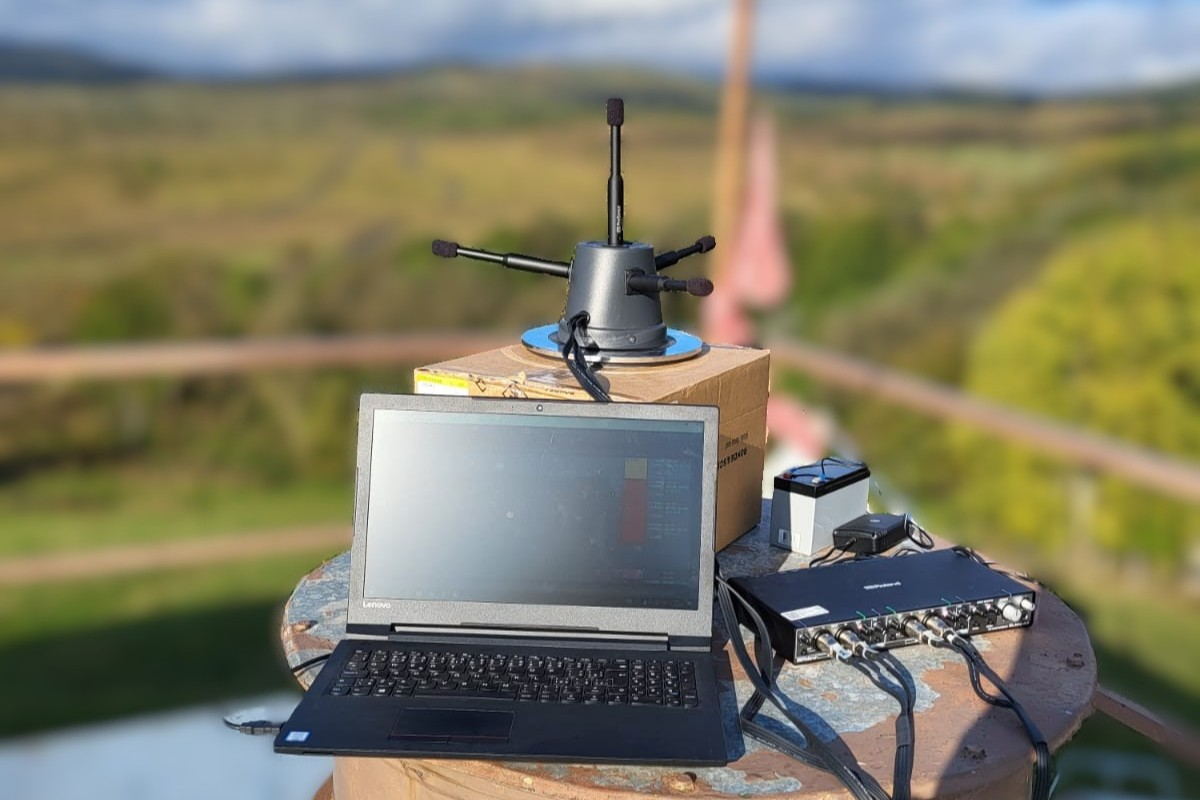
\includegraphics[width=\textwidth,height=38mm,keepaspectratio]{figs/sec2_measuring_setup.jpg}
      \par\vspace{1mm}
      \begin{itemize}\scriptsize
        \item Two days, one \textbf{152\,mm} self-propelled howitzer.
        \item Station 1--2\,km from the impact area; guns $\approx$5--10\,km away.
        \item 4 synchronized mics (PreSonus PRM1), Roland Rubix 44; 16\,bit, 22.05\,kHz.
      \end{itemize}
    \end{column}
    \begin{column}{0.57\textwidth}
      \vspace{-1mm}
      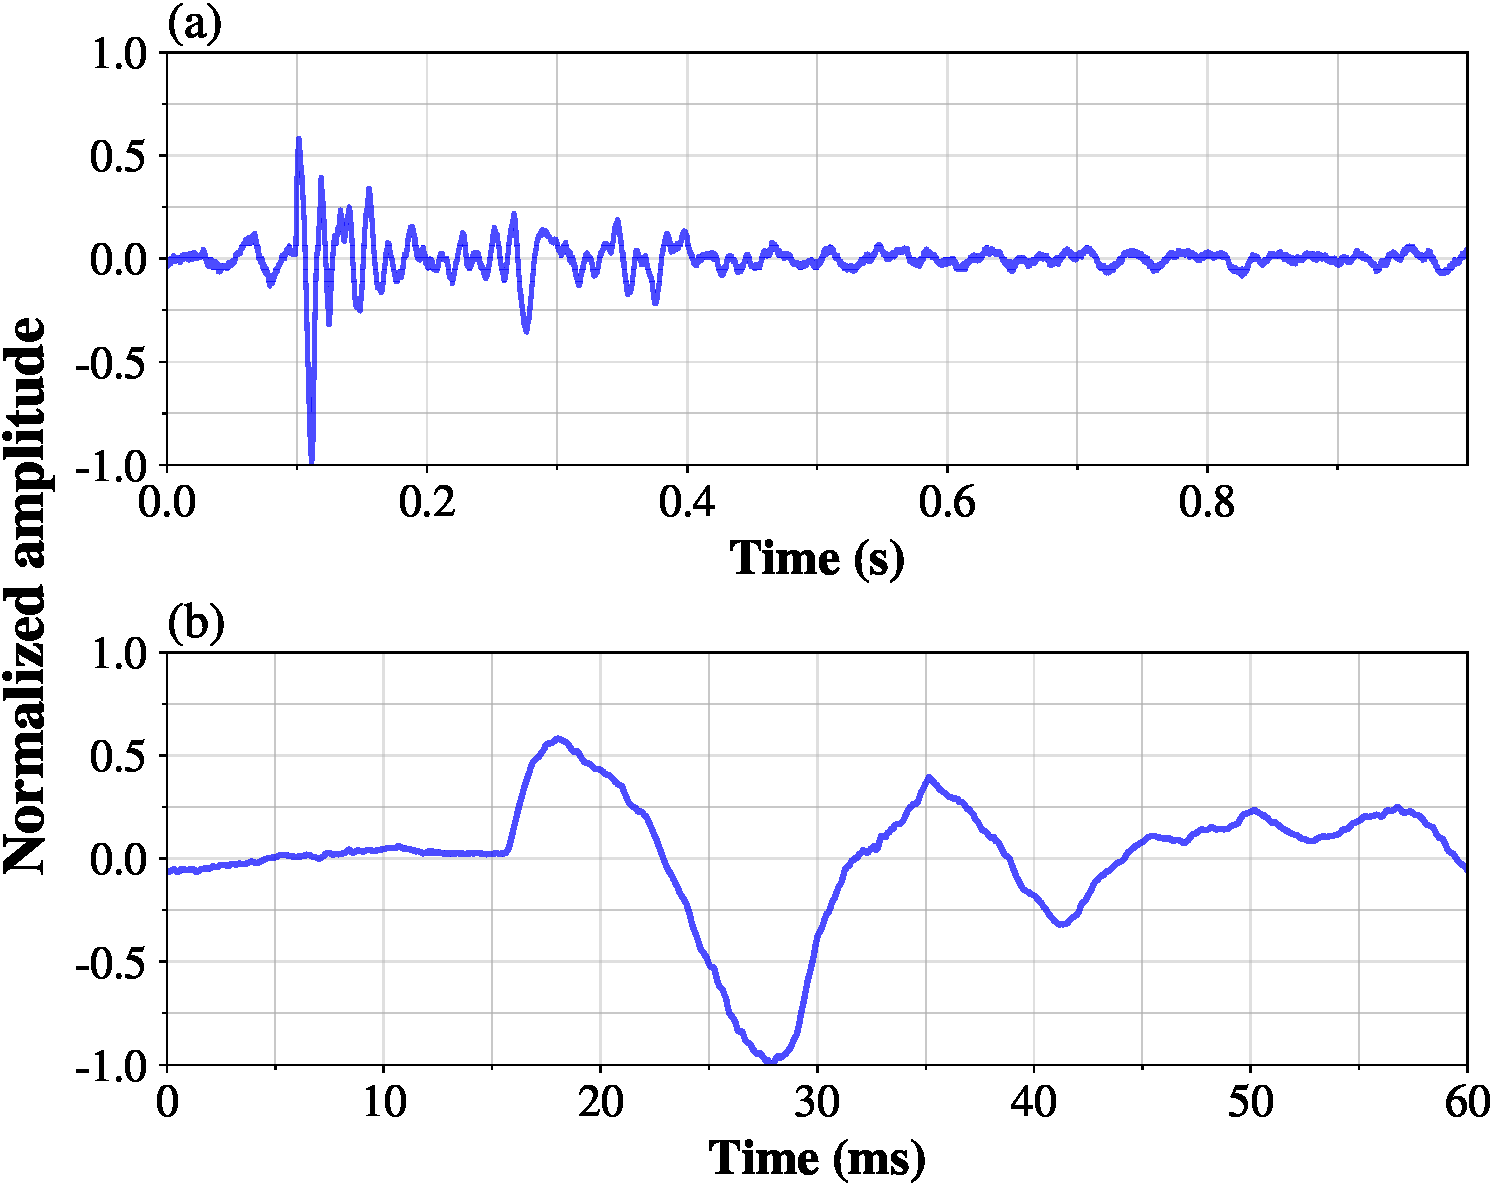
\includegraphics[width=\textwidth,height=56mm,keepaspectratio]{figs/sec2_waveform_combined.pdf}
      \par\vspace{1mm}
      {\scriptsize\color{ink!70} (a) launch recording; (b) the 60\,ms analysis window
       cut around the detected peak.}
    \end{column}
  \end{columns}
      \note{
\textbf{[3:50--4:50]}\par\medskip
    The data come from real artillery measurements. //\par\medskip
    This is our recording station. // Four synchronized microphones on one mount, an
    audio interface and a laptop. //\par\medskip
    We recorded for two days, with one type of gun -- a 152 millimetre self-propelled
    howitzer. // The station was one to two kilometres from the impact area, and the guns
    fired from about five to ten kilometres away. //\par\medskip
    On the right is one launch. // Below it, you can see the sixty millisecond window
    that the classifier actually sees. // Thirty percent of it is before the peak, and
    seventy percent after it. //
  }
\end{frame}

\begin{frame}{Labelled corpus and event-level split}
  \begin{columns}[c,onlytextwidth]
    \begin{column}{0.56\textwidth}
      \centering\footnotesize
      \begin{tabular}{@{}lrrrr@{}}
        \toprule
         & & \multicolumn{3}{c}{Samples}\\
        \cmidrule(l){3-5}
        Subset & Events & Train & Val. & Test\\
        \midrule
        \hl{Artillery launch} & \hl{50} & \hl{128} & \hl{8} & \hl{10}\\
        Impulsive noise   & 706 & 457 & 109 & 140\\
        Small-arms shots  &  85 &  49 &  18 &  18\\
        \midrule
        Total             & \textbf{841} & \textbf{634} & \textbf{135} & \textbf{168}\\
        \bottomrule
      \end{tabular}
    \end{column}
    \begin{column}{0.42\textwidth}
      \begin{itemize}\small
        \item Non-launch: false-trigger candidates -- door impacts, shouts, bells,
              \textbf{small-arms gunshots} as hard negatives.
        \item Split \textbf{by event}: the four channels of one shot never cross
              partitions.
        \item Training uses all 4 channels (launch share 20\,\%, class-weighted loss);
              validation and test use one.
      \end{itemize}
    \end{column}
  \end{columns}
      \note{
\textbf{[4:50--5:40]}\par\medskip
    This is the whole labelled corpus -- eight hundred and forty-one events. //\par\medskip
    Fifty of them are artillery launches. // The rest are things that can also fire the
    trigger -- doors, shouts, bells, and small-arms gunshots. // The gunshots are the
    hard cases, because they are impulsive too. //\par\medskip
    We split the data by event, not by recording. // So the four channels of one shot are
    never in training and test at the same time. //\par\medskip
    In training we use all four channels, and a class-weighted loss for the imbalance. //
    The test set has ten launches and one hundred and fifty-eight other events. //
  }
\end{frame}

\begin{frame}{Small positive class -- why, and how we handle it}
  \begin{columns}[T,onlytextwidth]
    \begin{column}{0.40\textwidth}
      \begin{block}{\faCrosshairs\enspace Why only 50 launches}
        \small
        \begin{itemize}\small
          \item Artillery cannot be recorded on demand -- only during a
                \textbf{live-fire exercise}, by arrangement with the military.
          \item The number of rounds was set by the exercise, \textbf{not by us}.
          \item Two recording days, one gun type.
        \end{itemize}
      \end{block}
    \end{column}
    \begin{column}{0.56\textwidth}
      {\small\bfseries\color{ctublue}How we limit the impact}
      \begin{itemize}\small
        \item \textbf{More views of each shot} -- all 4 synchronized channels in training,
              plus one noisy copy per SNR level.
        \item \textbf{No leakage} -- split by event, so no shot is in training and test.
        \item \textbf{Imbalance} -- hard negatives and a class-weighted loss (1\,:\,4).
        \item \textbf{Against overfitting} -- compact CNN (72\,k), dropout 0.5, early
              stopping on a separate validation set.
        \item \textbf{Honest numbers} -- test set used once; 5\,$\times$\,5 seeds;
              MCC instead of accuracy.
      \end{itemize}
    \end{column}
  \end{columns}
  \vfill
  {\small\color{ink!70} Still: 10 test launches and one gun type -- generalization to
   other calibres is untested.}
      \note{
\textbf{[5:40--6:40]}\par\medskip
    You may ask why we have only fifty launches. //\par\medskip
    Artillery is not something you can record whenever you want. // We could only record
    during a live-fire exercise, and it had to be arranged in advance. // The number of
    rounds was given by the exercise, not by us. //\par\medskip
    So we tried to get the most out of every shot. // In training we use all four
    microphone channels, and we add noisy copies. // We split by event, so no shot is in
    both training and test. // The network is small, with dropout and early stopping. //
    And every number is averaged over twenty-five runs. //\par\medskip
    Still -- ten test launches and one gun type is a real limitation. //
  }
\end{frame}

% ===========================================================================
\section{Method}

\begin{frame}{MFCC front end and compact CNN}
  \begin{columns}[T,onlytextwidth]
    \begin{column}{0.36\textwidth}
      \small\textbf{MFCC}
      \begin{itemize}\small
        \item 2.5\,ms frames, 1\,ms hop, Hamming
        \item 512-point FFT, 40 mel filters
        \item first 12 coefficients
        \item input tensor \textbf{$58\times12$}
      \end{itemize}
      \vspace{2mm}
      \small\textbf{Training}
      \begin{itemize}\small
        \item Adam, binary cross-entropy
        \item early stopping on validation loss
      \end{itemize}
    \end{column}
    \begin{column}{0.62\textwidth}
      \centering
      \begin{tikzpicture}[
          lay/.style={draw=ctublue,thick,rounded corners,fill=ctublue!8,
                      minimum width=40mm,minimum height=6.2mm,font=\small,align=center},
          pool/.style={lay,draw=ink!35,fill=ink!5,text=ink!75},
          outl/.style={lay,draw=accent,fill=accent!8,text=accent,font=\small\bfseries},
          dim/.style={font=\scriptsize\color{ink!60},anchor=west},
          ar/.style={-{Latex[length=1.5mm]},draw=gray,semithick},
          node distance=2.4mm
        ]
        \node[pool] (in) {MFCC input};
        \node[lay,below=of in] (c1) {Conv2D, 32 $\times$ ($3\times3$), ReLU};
        \node[pool,below=of c1] (p1) {MaxPool $2\times2$};
        \node[lay,below=of p1] (c2) {Conv2D, 64 $\times$ ($3\times3$), ReLU};
        \node[pool,below=of c2] (p2) {MaxPool $2\times2$};
        \node[lay,below=of p2] (d1) {Dense 64, ReLU + Dropout 0.5};
        \node[outl,below=of d1] (o) {Dense 1, sigmoid};
        \foreach \a/\b in {in/c1,c1/p1,p1/c2,c2/p2,p2/d1,d1/o} \draw[ar] (\a) -- (\b);
        \node[dim] at ($(in.east)+(2mm,0)$) {$58\times12\times1$};
        \node[dim] at ($(c1.east)+(2mm,0)$) {$56\times10\times32$};
        \node[dim] at ($(p1.east)+(2mm,0)$) {$28\times5\times32$};
        \node[dim] at ($(c2.east)+(2mm,0)$) {$26\times3\times64$};
        \node[dim] at ($(p2.east)+(2mm,0)$) {$13\times1\times64 \rightarrow 832$};
        \node[dim] at ($(d1.east)+(2mm,0)$) {64};
        \node[dim] at ($(o.east)+(2mm,0)$) {1};
      \end{tikzpicture}
      \par\vspace{1mm}
      {\scriptsize\color{ink!70}\textbf{72\,193} trainable parameters}
    \end{column}
  \end{columns}
      \note{
\textbf{[6:40--7:40]}\par\medskip
    Now the method. //\par\medskip
    From each window we compute MFCCs. // We use very short frames -- two and a half
    milliseconds, with a one millisecond step -- because the event is short and changes
    fast. // We keep twelve coefficients, so each event becomes a small matrix, fifty-eight
    by twelve. //\par\medskip
    The classifier is a small CNN. // Two convolution blocks, each with max pooling, then
    one dense layer with dropout, and a sigmoid output. //\par\medskip
    In total it has about seventy-two thousand parameters. // That is small enough for a
    microcontroller. //
  }
\end{frame}

\begin{frame}{Robustness training}
  \centering
  \begin{tikzpicture}[twoways]
    \node[blk] (b1) at (0,0) {waveform};
    \node[sum=accent] (bs) at (2.2,0) {};
    \node[blk] (b2) at (4.4,0) {MFCC};
    \node[blk] (b3) at (6.6,0) {CNN};
    \noisesrc{bn}{$(bs)+(0,9.5mm)$}{accent}
    \node[font=\scriptsize\color{accent},anchor=west] at ($(bn.east)+(1.5mm,0)$)
      {additive noise, 30 / 20 / 10 / 5\,dB SNR};
    \draw[ar] (b1) -- (bs); \draw[ar] (bs) -- (b2); \draw[ar] (b2) -- (b3);
    \draw[ar] (bn) -- (bs);
    \node[why] (bw) at ($(b3.east)+(5mm,0)$)
      {noise enters \textbf{before} the MFCC --\\ the way it reaches the real sensor};
  \end{tikzpicture}
  \par\vspace{5mm}
  \raggedright
  \begin{itemize}
    \item \textbf{Expanded non-launch corpus} -- small-arms shots and other impulsive
          sounds as hard negatives.
    \item \textbf{Class-weighted loss} for the 1\,:\,4 launch / non-launch imbalance.
    \item \textbf{Waveform-domain noise augmentation}, training split only -- the MFCCs
          are recomputed for every noisy copy.
  \end{itemize}
  \vfill
  {\scriptsize\color{ink!60} Control in the paper: the same noise added to the MFCC matrix
   instead does not give robustness (appendix).}
      \note{
\textbf{[7:40--8:30]}\par\medskip
    To make the classifier robust, we train it on noisy data. //\par\medskip
    We add noise to the training audio, at thirty down to five decibels, and only then
    compute the MFCCs. // That's how noise reaches the real sensor. //\par\medskip
    Together with that, we use a larger set of non-launch events, with gunshots as hard
    negatives, and a class-weighted loss for the imbalance. //
  }
\end{frame}

\begin{frame}{Evaluation protocol}
  \begin{itemize}
    \item Held-out test partition, used only for the final numbers.
    \item Noise added to the \textbf{waveform before MFCC extraction}, per event:
          \[ \sigma_n^2 = P_x \cdot 10^{-\mathrm{SNR}/10} \]
          at \textbf{30, 20, 10, 5\,dB} -- plus 0 and $-5$\,dB as a stress test,
          beyond the trigger's 5\,dB envelope.
    \item Peak detection and windowing re-run on the noisy signal.
    \item \textbf{5 training seeds $\times$ 5 noise seeds} = 25 runs per cell,
          mean $\pm$ std; threshold 0.5.
    \item Three regimes: \textbf{float32} and \textbf{int8} on the PC, int8 on the
          \textbf{ESP32-S3}.
    \item Main metric: Matthews correlation coefficient (MCC).
  \end{itemize}
      \note{
\textbf{[8:30--9:20]}\par\medskip
    How do we test it? //\par\medskip
    We take the held-out test set and add noise to the audio -- again before the MFCC,
    because that's what happens in the real sensor. // The noise level is set per event,
    from the power of the event itself. //\par\medskip
    We test thirty, twenty, ten and five decibels. // And then zero and minus five, which
    is already beyond what the trigger can handle. //\par\medskip
    Every number is an average over twenty-five runs -- five training seeds and five noise
    seeds. // And we report mainly the MCC, because the classes are imbalanced. //
  }
\end{frame}

% ===========================================================================
\section{Results}

\begin{frame}{Result 1 -- robustness at low SNR}
  \centering
  \begin{tikzpicture}
    \begin{axis}[snrslide,
        ymin=0.6,ymax=1.03,ytick={0.6,0.7,0.8,0.9,1.0},
        xmin=-0.3,xmax=6.3,
        xtick={0,1,2,3,4,5,6},xticklabels={clean,30,20,10,5,0,$-5$},
        xlabel={SNR (dB)},
        ylabel={int8 (--)}]
      % stress region: beyond the trigger's validated envelope
      \fill[ink!5] (axis cs:4.5,0.6) rectangle (axis cs:6.3,1.03);
      \node[font=\scriptsize\color{ink!55},anchor=south] at (axis cs:5.4,0.61)
        {beyond trigger envelope};
      \addplot[dim=gray3] coordinates {(0,1.000) (1,0.996) (2,0.988) (3,0.972) (4,0.956) (5,0.904) (6,0.716)}
        node[lbl=gray1] {recall};
      \addplot[dim=gray2] coordinates {(0,0.982) (1,0.982) (2,0.996) (3,0.985) (4,1.000) (5,1.000) (6,1.000)}
        node[lbl=gray1] {precision};
      \addplot[hot] coordinates {(0,0.990) (1,0.988) (2,0.992) (3,0.977) (4,0.976) (5,0.947) (6,0.833)}
        node[lbl=accent,font=\scriptsize\bfseries] {MCC};
    \end{axis}
  \end{tikzpicture}
  \par\vspace{1mm}
  {\scriptsize\color{ink!70} Precision stays \textbf{1.000} from 5\,dB down -- in heavy
   noise the model misses launches, it does not raise false alarms.
   float32 vs.\ int8: within $\pm0.02$ MCC, no consistent direction.}
      \note{
\textbf{[9:20--10:30]}\par\medskip
    This is the main result -- the deployed model on the held-out test set. //\par\medskip
    In the trained range, from clean down to five decibels, the MCC stays between zero
    point nine eight and zero point nine nine. //\par\medskip
    In the grey area, beyond what the trigger can handle, it goes down slowly. // Zero
    point nine five at zero decibels, and zero point eight three at minus five. //\par\medskip
    But look at how it fails. // Precision stays at one. // Only recall drops. // So in
    very strong noise the model misses some launches -- but it does not give false alarms.
    // And no small-arms gunshot was ever classified as artillery. //\par\medskip
    Quantization to int8 made no real difference. //
  }
\end{frame}

\begin{frame}{Result 2 -- on the ESP32-S3}
  \begin{columns}[T,onlytextwidth]
    \begin{column}{0.48\textwidth}
      \begin{block}{Same answers as the PC}
        \small
        \hl{1\,171 of 1\,176} inferences bit-exact with PC int8.\\[2pt]
        The 5 others: scores at exactly 0.5 -- a legal one-bit rounding difference
        between TFLite and TFLite Micro kernels.
      \end{block}
      \vspace{2mm}
      \begin{block}{Latency}
        \small
        \hl{32.0\,ms} per MFCC segment (31.99--32.09\,ms), independent of noise.\\[2pt]
        {\scriptsize\color{ink!70}Classifier inference only -- MFCC computed on the host.}
      \end{block}
    \end{column}
    \begin{column}{0.48\textwidth}
      \centering\small
      \begin{tabular}{@{}lr@{}}
        \toprule
        TensorFlow Lite Micro, int8 & \\
        \midrule
        Model size       & 81\,400\,B\\
        \texttt{tensor\_arena} & 80\,KiB\\
        Flash -- code    & 201.5\,kB\\
        Flash -- data    & 144.0\,kB\\
        RAM              & 143.8\,kB\\
        \bottomrule
      \end{tabular}
      \par\vspace{3mm}
      {\scriptsize\color{ink!70} All 8 operators native in TFLite Micro;
       compute-heavy ones via ESP-NN kernels.}
    \end{column}
  \end{columns}
      \note{
\textbf{[10:30--11:30]}\par\medskip
    Finally, the microcontroller. //\par\medskip
    We sent all test inputs to the ESP32-S3, at all noise levels -- that's one thousand
    one hundred and seventy-six inferences. // One thousand one hundred and seventy-one
    gave exactly the same result as the PC. // The other five had a score of exactly zero
    point five, right on the decision boundary, where a one-bit rounding difference can
    flip the answer. //\par\medskip
    One inference takes thirty-two milliseconds. // Please note, that's only the network
    -- the MFCCs were computed on the host. //\par\medskip
    The model has about eighty kilobytes, and the whole firmware needs less than one
    hundred and fifty kilobytes of RAM. //
  }
\end{frame}

% ===========================================================================
\section{Discussion}

\begin{frame}{Limitations}
  \begin{itemize}
    \item \textbf{Stage 2 only} -- no continuous-stream false-trigger rate; results assume
          the trigger found the peak.
    \item \textbf{Small positive class} -- 50 launch events, one gun type (152\,mm);
          other calibres untested.
    \item \textbf{Synthetic Gaussian noise} -- added to the waveform, but no real field
          noise, propagation or device shift.
    \item \textbf{One event-level split}; no session-independent evaluation.
    \item \textbf{MFCC on the host} -- on-device MFCC, end-to-end latency and energy per
          decision are future work.
  \end{itemize}
      \note{
\textbf{[11:30--12:00]}\par\medskip
    Of course, there are limitations. //\par\medskip
    We evaluate only the classifier, not the full stream. // We have only fifty launches,
    and one type of gun. // And the noise is synthetic. //\par\medskip
    So these are the next steps for us. //
  }
\end{frame}

% ===========================================================================
\section{Conclusion}

\begin{frame}{Conclusion}
  \begin{itemize}
    \item A compact MFCC-CNN (72\,k parameters) works as the post-trigger stage of an
          embedded artillery launch detector.
    \item Trained with noise added to the waveform, it stays robust:
          \hl{MCC 0.99 at 30\,dB, 0.98 at 5\,dB}; precision 1.0 under heavy noise.
    \item int8 is performance-neutral; ESP32-S3 matches the PC, 32\,ms per inference.
  \end{itemize}
  \vfill
  \centering
  {\large Thank you -- questions?}\\[2mm]
  {\small\color{gray} maxamart@fel.cvut.cz}
      \note{
\textbf{[12:00--12:40]}\par\medskip
    To sum up. //\par\medskip
    A small CNN with seventy-two thousand parameters works well as the second stage of an
    artillery launch detector. //\par\medskip
    Trained with noise in the audio, it keeps an MCC of zero point nine eight at five
    decibels. //\par\medskip
    Quantization to int8 costs nothing, and it runs on an ESP32-S3 in thirty-two
    milliseconds. //\par\medskip
    Thank you for your attention. // I'm happy to take your questions. //
  }
\end{frame}

% ===========================================================================
\appendix

\begin{frame}{Appendix -- full held-out robustness table}
  \centering\scriptsize
  \begin{tabular}{@{}ccccccc@{}}
    \toprule
    SNR (dB) & Accuracy (\%) & Precision & Recall & F1 & MCC & MCC (float32)\\
    \midrule
    Clean & 99.88 $\pm$ 0.24 & 0.982 $\pm$ 0.037 & 1.000 $\pm$ 0.000 & 0.990 $\pm$ 0.019 & 0.990 $\pm$ 0.020 & 1.000 $\pm$ 0.000\\
    30 & 99.86 $\pm$ 0.26 & 0.982 $\pm$ 0.037 & 0.996 $\pm$ 0.020 & 0.988 $\pm$ 0.021 & \hl{0.988 $\pm$ 0.022} & 0.998 $\pm$ 0.011\\
    20 & 99.90 $\pm$ 0.22 & 0.996 $\pm$ 0.018 & 0.988 $\pm$ 0.033 & 0.992 $\pm$ 0.019 & 0.992 $\pm$ 0.020 & 0.993 $\pm$ 0.018\\
    10 & 99.74 $\pm$ 0.39 & 0.985 $\pm$ 0.034 & 0.972 $\pm$ 0.061 & 0.977 $\pm$ 0.035 & 0.977 $\pm$ 0.035 & 0.974 $\pm$ 0.039\\
    5 & 99.74 $\pm$ 0.42 & 1.000 $\pm$ 0.000 & 0.956 $\pm$ 0.071 & 0.976 $\pm$ 0.039 & \hl{0.976 $\pm$ 0.039} & 0.978 $\pm$ 0.036\\
    \midrule
    0$^{\mathrm{a}}$ & 99.43 $\pm$ 0.53 & 1.000 $\pm$ 0.000 & 0.904 $\pm$ 0.089 & 0.947 $\pm$ 0.049 & 0.947 $\pm$ 0.049 & 0.934 $\pm$ 0.045\\
    $-5^{\mathrm{a}}$ & 98.31 $\pm$ 1.01 & 1.000 $\pm$ 0.000 & 0.716 $\pm$ 0.170 & 0.823 $\pm$ 0.122 & 0.833 $\pm$ 0.107 & 0.820 $\pm$ 0.088\\
    \bottomrule
  \end{tabular}
  \par\vspace{2mm}
  {\scriptsize\color{ink!70} Deployed int8 classifier, mean $\pm$ std over 5 training and
   5 noise seeds. Test partition: 168 samples, 10 of them launches.
   $^{\mathrm{a}}$Beyond the trigger's validated 5\,dB envelope.}
\end{frame}

\begin{frame}{Appendix -- control: noise on the MFCC features}
  \centering
  \begin{tikzpicture}
    \begin{axis}[snrslide,
        xmin=-0.3,xmax=4.3,
        xtick={0,1,2,3,4},xticklabels={clean,30\,dB,20\,dB,10\,dB,5\,dB},
        ylabel={held-out int8 MCC (--)}]
      \addplot[dim=gray3] coordinates {(0,0.82) (1,0.77) (2,0.56) (3,0.37) (4,0.30)}
        node[lbl=gray1] {MFCC jitter};
      \addplot[dim=gray2] coordinates {(0,0.97) (1,0.95) (2,0.92) (3,0.85) (4,0.86)}
        node[lbl=gray1,yshift=-3pt] {jitter + waveform};
      \addplot[hot] coordinates {(0,0.99) (1,0.99) (2,0.99) (3,0.98) (4,0.98)}
        node[lbl=accent,font=\scriptsize\bfseries,yshift=3pt] {waveform noise (deployed)};
    \end{axis}
  \end{tikzpicture}
  \par\vspace{1mm}
  {\scriptsize\color{ink!70} Same network, three augmentation strategies; mean over 25 runs.
   At 5\,dB: jitter $0.30\pm0.21$, jitter\,+\,waveform $0.86\pm0.07$, waveform \hl{$0.98\pm0.04$}.\\
   Gaussian jitter on the precomputed MFCC matrix does not imitate noise that passes through the MFCC.}
\end{frame}

\begin{frame}{Appendix -- design choices}
  \begin{columns}[T,onlytextwidth]
    \begin{column}{0.48\textwidth}
      \small\textbf{Why supervised, not anomaly detection?}
      \begin{itemize}\small
        \item After the trigger, \emph{every} candidate is already anomalous against the
              background -- small-arms shots included.
        \item One-class SVM / isolation forest / autoencoder would flag a rifle shot as
              ``anomalous'' -- not the decision we need.
        \item They fit stage 1 (novelty detection) rather than stage 2.
      \end{itemize}
      \small\textbf{Why MFCC, not GTCC?}
      \begin{itemize}\small
        \item GTCC won in our gunshot study (IMEKO 2026); MFCC is standardized with mature
              embedded implementations.
      \end{itemize}
    \end{column}
    \begin{column}{0.48\textwidth}
      \small\textbf{Why 22.05\,kHz?}
      \begin{itemize}\small
        \item Launch energy lies well below the 11\,kHz Nyquist limit.
        \item Buffers and MFCC compute scale with $f_s$ -- 44.1\,kHz would spend RAM
              without adding usable signal.
      \end{itemize}
      \small\textbf{Why ESP32-S3?}
      \begin{itemize}\small
        \item Low cost, low power, widely available; ESP-NN accelerated kernels for
              TFLite Micro.
        \item A representative Edge-AI MCU -- not a claim about all embedded targets.
      \end{itemize}
    \end{column}
  \end{columns}
\end{frame}

\begin{frame}{Appendix -- the five ESP32 disagreements}
  \begin{itemize}
    \item All five: PC int8 score is \textbf{exactly 0.5} -- on the decision threshold.
    \item The model is very confident, so the output quantization is coarse:
          \textbf{one LSB spans 10.8 logit units}.
    \item TFLite and TFLite Micro kernels may round one LSB differently -- both legal.
    \item Platform behaviour is equivalent up to rounding at the boundary;
          1\,171 / 1\,176 bit-exact.
  \end{itemize}
\end{frame}

\begin{frame}{Appendix -- metrics}
  \begin{description}
    \item[Precision] share of predicted launches that are real launches (false alarms).
    \item[Recall] share of real launches that were detected (missed launches).
    \item[MCC] Matthews correlation coefficient -- uses the whole confusion matrix,
      robust to class imbalance; $+1$ perfect, $0$ random.
  \end{description}
  \[ \text{MCC} = \frac{TP\cdot TN - FP\cdot FN}
      {\sqrt{(TP+FP)(TP+FN)(TN+FP)(TN+FN)}} \]
  \vfill
  {\small\color{gray} Test partition: 10 launches vs.\ 158 non-launch -- accuracy alone
   would be 94\,\% for a model that never says ``launch''.}
\end{frame}

\end{document}
